% 生成最终的图象时把第一个文档类取消注释即可
\documentclass[10pt,varwidth]{standalone}
% \documentclass[12pt]{article}
% 1.必须添加varwidth选项,不然就会报错
\PassOptionsToPackage{quiet}{fontspec}
\usepackage{ctex}
% \usepackage{geometry}
% 必须要保证绘图的纸张足够的大
\usepackage[a4paper, left=2.5cm, right=2.5cm, top=2.5cm, bottom=2.5cm]{geometry}
\usepackage{xifthen}
\usepackage{xfp}
\usepackage{xcolor}
\usepackage{pgfplots}
\usepackage{pgfplotstable}
\pgfplotsset{compat=1.16}
% 2.引用的tikz库
\usetikzlibrary {matrix, chains, trees, decorations}
\usetikzlibrary {arrows.meta, automata,positioning}
\usetikzlibrary {decorations.pathmorphing, calc}
\usetikzlibrary {calligraphy}
\usetikzlibrary {backgrounds, mindmap,shadows}
\usetikzlibrary {patterns, quotes, 3d, shadows}
\usetikzlibrary {graphs, fadings, scopes}
\usetikzlibrary {arrows, shapes.geometric}
\usepgflibrary {shadings}

\tikzset{
    >={Latex[length=6mm, width=2mm]}
}



\begin{document}
\,

\,
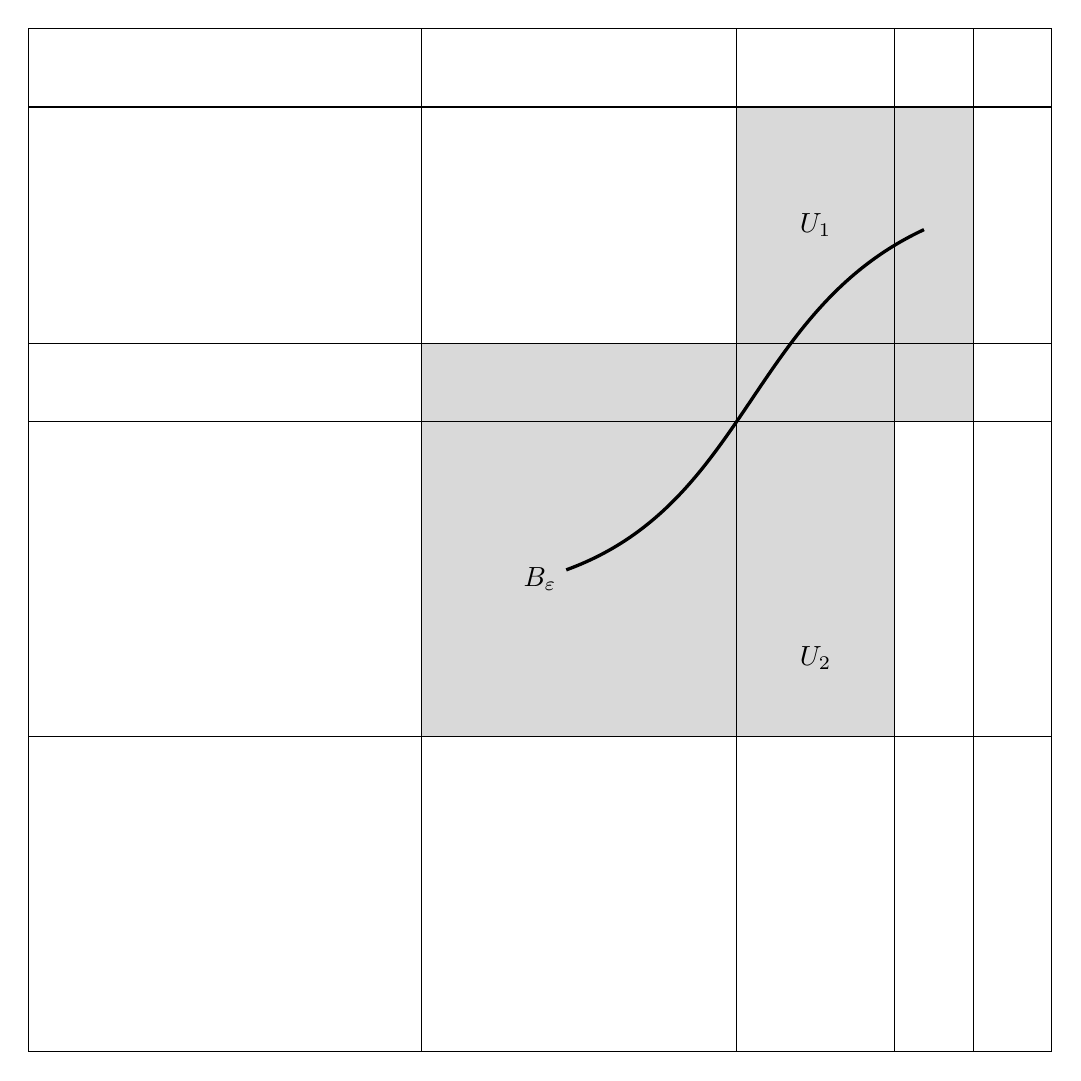
\begin{tikzpicture}
    % rectangle
    \draw (0, 0) rectangle (13, 13);
    % fill 
    \fill [gray!30] (12, 12) rectangle (9, 8);
    \fill [gray!30] (11, 9) rectangle (5, 4);
    % lines inside
    \foreach \x in {0, 5, 9, 11, 12, 13} {
        \draw (\x, 0) -- (\x, 13);
    }
    \foreach \y in {13, 12, 9, 8, 4, 0}{
        \draw (0, \y) -- (13, \y);
    }
    \node (A) at (11.5, 10.5) {};
    \node (B) at (6.5, 6) {$B_\varepsilon$};
    \node at (10, 10.5) {$U_1$};
    \node at (10, 5) {$U_2$};
    % arc
    \draw[very thick] (A) to[out=-155, in=20] (B);
\end{tikzpicture}
\end{document}